\documentclass[final,5p]{elsarticle}

% \documentclass[preprint,12pt]{elsarticle}

%% Use the option review to obtain double line spacing
%% \documentclass[authoryear,preprint,review,12pt]{elsarticle}

%% Use the options 1p,twocolumn; 3p; 3p,twocolumn; 5p; or 5p,twocolumn
%% for a journal layout:
% \documentclass[final,1p,times]{elsarticle}
%% \documentclass[final,1p,times,twocolumn]{elsarticle}
% \documentclass[final,3p,times]{elsarticle}
%% \documentclass[final,3p,times,twocolumn]{elsarticle}
% \documentclass[final,5p,times]{elsarticle}
%% \documentclass[final,5p,times,twocolumn]{elsarticle}
\usepackage[portuguese]{babel}

%% For including figures, graphicx.sty has been loaded in
%% elsarticle.cls. If you prefer to use the old commands
%% please give \usepackage{epsfig}

%% The amssymb package provides various useful mathematical symbols
\usepackage{amssymb}
\usepackage{amsmath}
\usepackage{multirow}
\usepackage{tabularx}

\usepackage{pgfplots}
\pgfplotsset{compat=1.18}
\usepgfplotslibrary{statistics}
\usepackage{pgfplotstable}

\usepackage{placeins}
\usepackage{hyperref}
\numberwithin{equation}{section}

\usepackage{algorithm}
\usepackage[noEnd=true, indLines=true]{algpseudocodex}
\algrenewcommand\algorithmicrequire{\textbf{Entrada:}}
\algrenewcommand\algorithmicwhile{\textbf{Enquanto}}
\algrenewcommand\algorithmicrepeat{\textbf{Repete}}
\algrenewcommand\algorithmicuntil{\textbf{Até}}
\algrenewcommand\algorithmicif{\textbf{Se}}
\algrenewcommand\algorithmicthen{\textbf{então}}
\algrenewcommand\algorithmicelse{\textbf{Caso contrário}}
\algrenewcommand\algorithmicensure{\textbf{Objetivo:}}
\algrenewcommand\algorithmicreturn{\textbf{Retorna:}}
\algrenewcommand\algorithmicdo{\textbf{faça}}
\algrenewcommand\algorithmicforall{\textbf{Para todos}}
\algnewcommand{\LineComment}[1]{\State \(\triangleright\) \textcolor{black!50}{\emph{#1}}}

\newcommand*{\squareb}{\textcolor{black}{\rule{0.5em}{0.5em}}}
\newcommand*{\squareg}{\textcolor{gray}{\rule{0.5em}{0.5em}}}

% \usepackage[fleqn]{nccmath}
% \usepackage{multicol}


%=========== Gloabal Tikz settings
% \pgfplotsset{compat=newest}
% \usetikzlibrary{math}
% \pgfplotsset{
%     height = 10cm,
%     width = 10cm,
%     tick pos = left,
%     legend style={at={(0.98,0.30)}, anchor=east},
%     legend cell align=left,
%     }
%  \pgfkeys{
%     /pgf/number format/.cd,
%     fixed,
%     precision = 1,
%     set thousands separator = {}
% }

%% The amsthm package provides extended theorem environments
%% \usepackage{amsthm}

%% The lineno packages adds line numbers. Start line numbering with
%% \begin{linenumbers}, end it with \end{linenumbers}. Or switch it on
%% for the whole article with \linenumbers.
%% \usepackage{lineno}

\usepackage{listings}
\usepackage{xcolor}

\definecolor{codegreen}{rgb}{0,0.6,0}
\definecolor{codegray}{rgb}{0.5,0.5,0.5}
\definecolor{codepurple}{rgb}{0.58,0,0.82}
\definecolor{backcolour}{rgb}{0.98,0.98,0.98}

\lstdefinestyle{mystyle}{
    backgroundcolor=\color{backcolour},
    commentstyle=\color{codegreen},
    keywordstyle=\color{magenta},
    numberstyle=\tiny\color{codegray},
    stringstyle=\color{codepurple},
    basicstyle=\ttfamily\footnotesize,
    breakatwhitespace=false,
    breaklines=true,
    captionpos=b,
    keepspaces=true,
    numbers=left,
    numbersep=5pt,
    showspaces=false,
    showstringspaces=false,
    showtabs=false,
    tabsize=2
}

\lstset{style=mystyle}

% \journal{Nuclear Physics B}

\begin{document}

\begin{frontmatter}

%% Title, authors and addresses

%% use the tnoteref command within \title for footnotes;
%% use the tnotetext command for theassociated footnote;
%% use the fnref command within \author or \address for footnotes;
%% use the fntext command for theassociated footnote;
%% use the corref command within \author for corresponding author footnotes;
%% use the cortext command for theassociated footnote;
%% use the ead command for the email address,
%% and the form \ead[url] for the home page:
%% \title{Title\tnoteref{label1}}
%% \tnotetext[label1]{}
%% \author{Name\corref{cor1}\fnref{label2}}
%% \ead{email address}
%% \ead[url]{home page}
%% \fntext[label2]{}
%% \cortext[cor1]{}
%% \affiliation{organization={},
%%             addressline={},
%%             city={},
%%             postcode={},
%%             state={},
%%             country={}}
%% \fntext[label3]{}

\title{Implementação de Modelo de Reservatório Bidimensional Incompressível Integrado com Facilidades de Produção\tnoteref{label_title}}
\tnotetext[label_title]{Relatório final da disciplina PP590A: Tópicos em Geoengenharia de Reservatórios.}

%% use optional labels to link authors explicitly to addresses:
%% \author[label1,label2]{}
%% \affiliation[label1]{organization={},
%%             addressline={},
%%             city={},
%%             postcode={},
%%             state={},
%%             country={}}
%%
%% \affiliation[label2]{organization={},
%%             addressline={},
%%             city={},
%%             postcode={},
%%             state={},
%%             country={}}

\author{Tiago C. A. Amorim\fnref{label_author}}
\tnotetext[label_author]{Atualmente cursando doutorado no Departamento de Engenharia de Petróleo da Faculdade de Engenharia Mecânica da UNICAMP (Campinas/SP, Brasil).}
\ead{t100675@dac.unicamp.br}
\affiliation[Tiago C. A. Amorim]{organization={Petrobras},%Department and Organization
addressline={Av. Henrique Valadares, 28},
city={Rio de Janeiro},
postcode={20231-030},
state={RJ},
country={Brasil}}

\begin{abstract}

    A modelagem integrada aumenta o custo computacional de simulações de fluxo, mas o seu uso enriquece a gama de análises que podem ser realizadas. Este trabalho mostra que ao integrar um simples modelo de fluxo em meio poroso incompressível com um sistema de produção, foi possível realizar análises de emissão de $CO_2$.

\end{abstract}


%%Graphical abstract
% \begin{graphicalabstract}
%\includegraphics{grabs}
% \end{graphicalabstract}

%%Research highlights
% \begin{highlights}
% \item Research highlight 1
% \item Research highlight 2
% \end{highlights}

\begin{keyword}
    Fluxo em Meio Poroso \sep Modelagem Integrada
%% keywords here, in the form: keyword \sep keyword

%% PACS codes here, in the form: \PACS code \sep code

%% MSC codes here, in the form: \MSC code \sep code
%% or \MSC[2008] code \sep code (2000 is the default)

\end{keyword}

\end{frontmatter}

%% \linenumbers

%% main text
\section{Introdução}

    Ao longo da disciplina de Modelagem Integrada foram abordados diferentes tópicos associados à modelagem de reservatórios e o sistema de produção: descrição de fluidos \emph{Black-oil}, fluxo em meios porosos, fluxo vertical multifásico, sistema de \emph{boosting}, problemas de garantia de escoamento, equipamentos de superfície e emissão de $CO_2$.
    Foram desenvolvidos diversos módulos em Python para modelar numericamente o comportamento de alguns dos mecanismos abordados. Este relatório descreve as funcionalidades implementadas e como foi realizada a integração destes módulos para chegar ao modelo integrado proposto.

\section{Implementação}

    Diversos módulos de cálculo foram criados. Cada um com foco em um dos assuntos abordados nas aulas. Buscou-se deixar os módulos como objetos independentes, e assim facilitar o desenvolvimento de novas funcionalidades.

    \subsection{Propriedades de Fluido}

        A descrição do fluido foi implementada na classe \textbf{PVT} do módulo \emph{pvt.py}. Foram utilizadas as correlações de Standing\cite{standing1952volumetric} para estimativa de parâmetros de óleo e gás\footnote{As correlações utilizadas foram suprimidas deste relatório para não sobrecarregá-lo de informações, e podem ser encontradas em \cite{rosa2006engenharia}.}:

        \begin{itemize}
            \item Fator volume de formação ($Bg$ e $Bo$).
            \item Razão de solubilidade do óleo ($Rs$).
            \item Viscosidade ($\mu_g$ e $\mu_o$).
        \end{itemize}

        As propriedades são basicamente função da densidade do óleo ($^oAPI$), densidade do gás ($dg$), razão gás-óleo ($RGO$), pressão e temperatura. Outras grandezas auxiliares, necessárias nas estimativas das grandezas de interesse, são calculadas com correlações de Standing (eg.: compressibilidade do óleo).

        As propriedades da água são assumidas constantes e são diretamente fornecidas pelo usuário.

        Este módulo permite ao usuário fornecer um valor de fração de água ($wcut$) e pedir valores de densidade média ($\rho$) e viscosidade média ($\mu$). Os valores são médias ponderadas pela fração de água.

        Também existe a possibilidade de solicitar o uso da correlação de Rønningsen para estimar a viscosidade da mistura água-óleo considerando a formação de emulsões\cite{doi:10.1021/ef00041a001}:

        \begin{align}
            \ln \frac{\mu_{mix}}{\mu_o} &= k_1 + k_2 \, T + k_3 \, wcut  + k_4 \, T \, wcut
        \end{align}

        Onde $\mu_{mix}$ é a viscosidade da emulsão, $wcut$ é a fração de água e $T$ é a temperatura (em $^oC$). Os valores de $k_i$ são função da taxa de cisalhamento do fluido (Tabela \ref{tab:ronningsen}):

        \begin{align}
            \dot{\gamma} &= \frac{32 Q}{\pi d^3}
        \end{align}

        \begin{table}[ht]
            \centering
            \begin{tabular}{c|ccc}
                $\dot{\gamma}$ [$s^{-1}$] & 30 & 100 & 500 \\
                 \hline
                 $k_1$ & 0.01334 & 0.0412 & -0.06671 \\
                 $k_2$ & -0.003801 & -0.002605 & -0.000775 \\
                 $k_3$ & 4.338 & 3.841 & 3.484 \\
                 $k_4$ & 0.02698 & 0.02497 & 0.005 \\
            \end{tabular}
            \caption{Coeficientes da correlação de Rønningsen.}
            \label{tab:ronningsen}
        \end{table}

        Para taxas de cisalhamento diferentes das tabeladas, foi utilizada uma interpolação linear.

        Um pequeno ajuste foi realizado na formulação de Rønningsen. Para manter coerência com o cenário em que existe 100\% de óleo ($wcut=0$), o valor mínimo de $\frac{\mu_{mix}}{\mu_o}$ é igual à unidade (ver trecho reto para valores baixos de $wcut$ nas curvas da Figura \ref{fig:emulsao}).

        \begin{figure}[hbt!]
            \begin{tikzpicture}
                \begin{axis}[
                    grid=both,
                    xlabel = {Corte de água},
                    ylabel = {$\mu_{emuls\tilde{a}o}$ [cP]},
                    legend style={at={(0.90,0.85)}, anchor=east, font=\footnotesize},
                    ]
                    \addplot[color=blue, solid, thick] table [x=WCUT, y=U_1cP] {emulsao.txt};
                    \addplot[color=black, solid, thick] table [x=WCUT, y=U_10cP] {emulsao.txt};
                    \legend{Óleo 1 cP, Óleo 10 cP};
                \end{axis}
            \end{tikzpicture}
            \caption{Estimativa de viscosidade de emulsão a 50 $^oC$ e $\dot{\gamma} = 100\,s^{-1}$.}
            \label{fig:emulsao}
        \end{figure}

        A inversão de fases é estimada com a correlação de Arirachakaran\cite{10.2118/18836-MS}:

        \begin{align}
            \varepsilon_w &= \max \left(0.15; 0.5 - 0.1108 \log_{10} \frac{\mu_o}{\mu_{w,ref}}\right)
        \end{align}

        Onde $\varepsilon_w$ é o valor de fração de água a partir da qual há inversão de fase e $\mu_{w,ref}$ é uma viscosidade de água de referência, igual a 1 cP. Para valores de fração de água maiores que $\varepsilon_w$ a viscosidade da mistura água-óleo é a média ponderada pela fração de água dos respectivos valores.

    \subsection{Fluxo em Meio Poroso}

        As equações que regem o problema de fluxo em meio poroso derivam fundamentalmente da equação de conservação de massa \ref{eq:consmassa} e da equação de fluxo em meio poroso \ref{eq:darcy}, a lei de Darcy \cite{dake1983fundamentals}.

        \begin{align}
            &\sum_{p} \nabla \cdot  (y_{cp} \rho_p v_p) + \sum_{p} (y_{cp} \rho_p q_p) + \sum_{p} \frac{\partial}{\partial t} \left( \phi y_{cp} \rho_p S_p\right) = 0 \label{eq:consmassa} \\
            &v_p = - \frac{k k_{rp}}{\mu_p} \left( \frac{\partial p_p}{\partial x} - \gamma_p \frac{\partial D}{\partial x} \right) = - \frac{k k_{rp}}{\mu_p} \left( \frac{\partial \Phi_p}{\partial x} \right)\label{eq:darcy}
        \end{align}

        A maioria dos simuladores de fluxo comerciais utilizam diferenças finitas \cite{computer2022cmg}\cite{schlumberger2009technical}. Podemos acoplar as equações \ref{eq:consmassa} e \ref{eq:darcy}, e aplicar uma discretização no tempo ($\Delta t$) e no espaço ($\Delta x$) para um volume de controle ($V = \Delta x \Delta y \Delta z$)\footnote{Usualmente chamado de célula.}. A forma unidimensional desta equação discretizada é apresentada em \ref{eq:geralumd}.

        \begin{align}
            \sum_{p} & \left( \frac{\Delta y \Delta z}{\Delta x} y_{cp} \rho_p \frac{k k_{rp}}{\mu_p} \right)_{i+\tfrac{1}{2}} (\Phi_{p,i+1} - \Phi_{p,i})  \nonumber \\
            & + \left( \frac{\Delta y \Delta z}{\Delta x} y_{cp} \rho_p \frac{k k_{rp}}{\mu_p} \right)_{i-\tfrac{1}{2}} (\Phi_{p,i-1} - \Phi_{p,i}) \nonumber \\
            & + q_{cp}^{w} = \frac{1}{\Delta t} \sum_{p} (V \phi y_{cp} \rho_p S_p)_i^{t_i+\Delta t} - (V \phi y_{cp} \rho_p S_p)_i^{t_i} \label{eq:geralumd}
        \end{align}

        Na sua forma mais geral o problema de fluxo em meio poroso precisa ser resolvido para cada um dos componentes que constituem as fases envolvidas. É comum utilizar uma abordagem simplificada, em que poucos componentes são utilizados para representar os fluidos envolvidos. Esta simplificação é usualmente aplicada quando as trocas de fase são \emph{bem comportadas} e passíveis de serem representadas por um conjunto de tabelas, em substituição às equações de estado. Esta abordagem é conhecida como \emph{Black-Oil}.

        As equações também se simplificam ao substituir as densidades ($\rho_p$) e concentrações de componentes ($y_{cp}$) pelo fator volume de formação da fase ($B$) e as relações volumétricas entre as fases e os componentes ($R$)\footnote{Maiores detalhes em \cite{dake1983fundamentals}.}.

        Quando apenas água e óleo estão envolvidos na simulação, duas equações de conservação de massa são necessárias. Como a soma das saturações é igual à unidade ($S_w + S_o = 1$) e negligenciando a tensão interfacial entre a água e o óleo ($p_o = p_w = p$), para cada célula é preciso resolver apenas as variáveis $p$ e $S_w$:

        \begin{align}
            &\left( \frac{\Delta y \Delta z}{\Delta x} \lambda_w \right)_{i+\tfrac{1}{2}} (p_{i+1} - p_{i} - \gamma_w \Delta D_{i+\tfrac{1}{2}})  \nonumber \\
            &+ \left( \frac{\Delta y \Delta z}{\Delta x} \lambda_w \right)_{i-\tfrac{1}{2}} (p_{i-1} - p_{i} - \gamma_w \Delta D_{i-\tfrac{1}{2}}) \nonumber \\
            &  = \frac{1}{\Delta t} \left(\frac{V \phi S_w}{B_w}\right)_i^{t_i+\Delta t} - \left(\frac{V \phi S_w}{B_w}\right)_i^{t_i} + q^{std}_w \label{eq:blackoilumdw} \\
            &\left( \frac{\Delta y \Delta z}{\Delta x} \lambda_o \right)_{i+\tfrac{1}{2}} (p_{i+1} - p_{i} - \gamma_o \Delta D_{i+\tfrac{1}{2}})  \nonumber \\
            &+ \left( \frac{\Delta y \Delta z}{\Delta x} \lambda_o \right)_{i-\tfrac{1}{2}} (p_{i-1} - p_{i} - \gamma_o \Delta D_{i-\tfrac{1}{2}}) \nonumber \\
            &  = \frac{1}{\Delta t} \left(\frac{V \phi (1-S_w)}{B_o}\right)_i^{t_i+\Delta t} - \left(\frac{V \phi (1-S_w)}{B_o}\right)_i^{t_i} + q^{std}_o \label{eq:blackoilumdo}
        \end{align}

        \noindent com:
        \begin{align}
            \lambda_p = \frac{k k_{rp}}{B_p \mu_p} \nonumber
        \end{align}

        Observa-se que a pressão ($p$) e a saturação de água ($S_w$) da i-ésima célula tem influência apenas na própria célula e nas células vizinhas. Desta forma, a matriz dos coeficientes deste problema tem termos não nulos em três \emph{bandas} ao redor da diagonal principal. Para modelos bi e tridimensionais são adicionados novos termos fora da diagonal principal.

        No módulo \emph{reservoir.py} foi implementado o problema de fluxo em meio poroso bidimensional, incompressível e plano. Existem poços apenas em duas posições: injetor de água controlado por vazão especificada na célula [1,1] e produtor controlado por pressão de fundo na célula [$n_i$,$n_j$].

        As propriedades de fluido ($Bo$, $Bw$, $\mu_o$ e $\mu_w$) são constantes. O meio poroso também é incompressível, mas é possível definir valores de propriedade de rocha ($\phi$ e $k$) por célula.

        Foram implementadas funções de permeabilidade relativa com as correlações de Corey\cite{1570009749409873792}. As permeabilidades relativas foram implementadas na classe \textbf{Corey} no módulo \emph{relative\_permeability.py}.

        Em uma simulação \emph{Black-Oil} com água e óleo, a simulação de fluxo parte de um conjunto de valores de $p$ e $S_w$ no tempo inicial, para cada uma das células, e uma série de controles de produção ($q^{std}_p$). O simulador precisa resolver o conjunto de equações não lineares \ref{eq:blackoilumdw} e \ref{eq:blackoilumdo} a cada passo de tempo.

        Foi implementada a formulação implícita para resolver o problema de fluxo em meio poroso. A implementação mais conhecida para resolver este conjunto de equações não lineares é o Método de Newton-Raphson. Para sistemas incompressíveis (onde $\phi$, $B$ e $\mu$ são constantes) este conjunto de equações é \emph{fracamente} não linear, e apenas os valores de $k_{ro}$ e $k_{rw}$ são função das variáveis de estado. O conjunto de equações resultantes pode ser resolvido adequadamente com o Método do Ponto Fixo\cite{burden2016analise}. As equações são resolvidas como um conjunto de equações lineares de modo iterativo, isto é, utilizando o resultado de uma iteração como dado de entrada para resolver os termos $k_{ro}$ e $k_{rw}$ da próxima iteração, até que a convergência é atingida.

        O controle do tamanho tamanho do passo de tempo de cada iteração é feito de forma simplificada. O usuário precisa fornecer valores de máxima variação de saturação de água e de pressão entre os passos de tempo. Quando algum dos limites não é observado, o passo de tempo é reduzido à metade e a simulação do tempo \emph{atual} é feita novamente. Caso as máximas variações sejam atendidas, o simulador irá incrementar o passo de tempo para a próxima iteração em 20\%. O usuário também pode informar valores mínimo e máximo dos passos de tempo.

        Foi observado que este sistema incompressível tem dificuldades de convergência no primeiro passo de tempo da simulação. O problema está associado ao fato de que a célula em que o injetor de água está conectado tem saturação igual à saturação de água conata. Nesta situação a permeabilidade relativa da água é nula. Como o meio poroso é incompressível, nos primeiros passos de tempo é comum serem observados valores muito alto de pressão nesta célula e nas vizinhas. Este efeito é maior em modelos com células menores e altas vazões de injeção de água.
        Para evitar este efeito indesejado, foi implementada a opção de incrementar a saturação de água no tempo inicial desta célula. Esta alteração tem pouco ou nenhum impacto nos demais resultados (Figura \ref{fig:ajusteswprod}), e evita valores de pressão anormais nos primeiros passos de tempo (Figura \ref{fig:ajustesw}). Para o problema proposto foi utilizado um valor de 5\%.

        \begin{figure}[hbt!]
            \begin{tikzpicture}
                \begin{axis}[
                    grid=both,
                    xlabel = {Tempo [d]},
                    ylabel = {Pwf produtor [bar]},
                    legend style={font=\footnotesize},
                    % ymax=2100.,
                    % ymin=900.,
                    xmax=82.,
                    xmin=-2.,
                    ]
                    \addplot[color=black, solid, thick] table [x=Time_d, y=PwfProd_bar] {results_1stSw_0pc.txt};
                    \addplot[color=blue, solid, thick] table [x=Time_d, y=PwfProd_bar] {results_1stSw_1pc.txt};
                    \addplot[color=red, solid, thick] table [x=Time_d, y=PwfProd_bar] {results_1stSw_2pc.txt};
                    \addplot[color=green, solid, thick] table [x=Time_d, y=PwfProd_bar] {results_1stSw_3pc.txt};
                    \addplot[color=gray, solid, thick] table [x=Time_d, y=PwfProd_bar] {results_1stSw_4pc.txt};
                    \addplot[color=yellow, solid, thick] table [x=Time_d, y=PwfProd_bar] {results_1stSw_5pc.txt};
                    \addplot[color=purple, solid, thick] table [x=Time_d, y=PwfProd_bar] {results_1stSw_6pc.txt};
                    \addplot[color=cyan, solid, thick] table [x=Time_d, y=PwfProd_bar] {results_1stSw_7pc.txt};
                    \legend{$\Delta S_w=0\%$,$\Delta S_w=2\%$,$\Delta S_w=2\%$,$\Delta S_w=3\%$,$\Delta S_w=4\%$,$\Delta S_w=5\%$,$\Delta S_w=6\%$,$\Delta S_w=7\%$};
                \end{axis}
            \end{tikzpicture}
            \caption{Efeito na pressão de fundo do produtor de modificar a saturação inicial de água da célula do injetor de água.}
            \label{fig:ajusteswprod}
        \end{figure}

        \begin{figure}[hbt!]
            \begin{tikzpicture}
                \begin{axis}[
                    grid=both,
                    xlabel = {Tempo [d]},
                    ylabel = {Pwf injetor [bar]},
                    legend style={font=\footnotesize},
                    ymax=2100.,
                    ymin=900.,
                    xmax=82.,
                    xmin=-2.,
                    ]
                    \addplot[color=black, solid, thick] table [x=Time_d, y=PwfInj_bar] {results_1stSw_0pc.txt};
                    \addplot[color=blue, solid, thick] table [x=Time_d, y=PwfInj_bar] {results_1stSw_1pc.txt};
                    \addplot[color=red, solid, thick] table [x=Time_d, y=PwfInj_bar] {results_1stSw_2pc.txt};
                    \addplot[color=green, solid, thick] table [x=Time_d, y=PwfInj_bar] {results_1stSw_3pc.txt};
                    \addplot[color=gray, solid, thick] table [x=Time_d, y=PwfInj_bar] {results_1stSw_4pc.txt};
                    \addplot[color=yellow, solid, thick] table [x=Time_d, y=PwfInj_bar] {results_1stSw_5pc.txt};
                    \addplot[color=purple, solid, thick] table [x=Time_d, y=PwfInj_bar] {results_1stSw_6pc.txt};
                    \addplot[color=cyan, solid, thick] table [x=Time_d, y=PwfInj_bar] {results_1stSw_7pc.txt};
                    \legend{$\Delta S_w=0\%$,$\Delta S_w=2\%$,$\Delta S_w=2\%$,$\Delta S_w=3\%$,$\Delta S_w=4\%$,$\Delta S_w=5\%$,$\Delta S_w=6\%$,$\Delta S_w=7\%$};
                \end{axis}
            \end{tikzpicture}
            \caption{Efeito na pressão de fundo do injetor de modificar a saturação inicial de água da célula do injetor de água.}
            \label{fig:ajustesw}
        \end{figure}

    \subsection{Fluxo Vertical Multifásico}

        Forma implementadas quatro classes no módulo \emph{flow.py}. Os cálculos de fluxo vertical multifásico são realizados na classe mais básica (\textbf{SubFlowElement}), que representa um trecho de tubulação, com diâmetro e inclinação constante. Este elemento utiliza o módulo \emph{pvt.py} para estimar as propriedades de fluido. Foram consideras as formas de balanço de massa e energia de fluidos quasi-incompressíveis.

        A perda de pressão no elemento pode ser calculada em ambas direções, i.e., alimentando as condições de entrada ($p_a$: pressão de entrada) e calculando as condições de saída ($p_b$: pressão de saída), ou o inverso:

        \begin{align}
            p_a - p_b = \rho g \left( (z_a - z_b) + H_L + \frac{v^2_b - v^2_a}{2 g}\right)
        \end{align}

        O termo de perda de carga por fricção ($H_L$) utiliza a formulação de Colebrook-White para o cálculo do fator de fricção ($f$) quando o número de Reynolds ($Re$) é maior que 4000. Para evitar descontinuidades, nos casos em que o número de Reynolds fica entre o fluxo laminar ($Re \leq 2100$) e o fluxo turbulento ($Re \geq 4000$), é aplicada uma correlação linear entre os valores de $f$ calculados para fluxo laminar e turbulento (Figura \ref{fig:friccao}).

        \begin{figure}[hbt!]
            \begin{tikzpicture}
                \begin{semilogxaxis}[
                    grid=both,
                    xlabel = {Número de Reynolds},
                    ylabel = {$f$},
                    legend style={at={(0.90,0.85)}, anchor=east, font=\footnotesize},
                    ]
                    \addplot[color=black, solid, smooth, thick] table [x=Reynold, y=f] {friccao_laminar.txt};
                    \addplot[color=blue, solid, smooth, thick] table [x=Reynold, y=f] {friccao_turbulento.txt};
                    \addplot[color=red, solid, smooth, thick] table [x=Reynold, y=f] {friccao_transicao.txt};
                    \addplot[color=black, dashed, smooth, thick] table [x=Reynold, y=f] {friccao_laminar_trans.txt};
                    \addplot[color=blue, dashed, smooth, thick] table [x=Reynold, y=f] {friccao_turbulento_trans.txt};
                    \legend{Laminar, Turbulento, Transição};
                \end{semilogxaxis}
            \end{tikzpicture}
            \caption{Proposta de cálculo do fator de fricção na região de transição.}
            \label{fig:friccao}
        \end{figure}

        Não foram implementadas correlações para troca de temperatura. Todo o cálculo é realizado assumindo temperatura constante por elemento. Também não foi implementado o cálculo de fluxo com gás livre, de modo que apenas água e óleo podem existir no sistema.

        O termo de ganho de energia com turbomáquinas foi deliberadamente retirado porque foi criada uma classe específica para representar uma bomba elétrica submersível (\textbf{ESP}). Não foram implementadas tabelas de eficiências de bomba. Um objeto \textbf{ESP} apenas recebe um valor de incremento de pressão e um valor de eficiência. O incremento de pressão é adicionado nos cálculos do fluxo vertical multifásico no ponto em que o usuário colocar a bomba. Um segundo comando realiza os cálculos da potência necessária para aplicar o incremento de pressão ao fluido em questão.

        Para levar em conta a variação na viscosidade da mistura água+óleo na eficiência da bomba, foi assumida\footnote{Esta correlação foi assumida sem nenhuma base científica. Foi utilizada apenas para que a viscosidade da mistura tenha algum impacto na demanda energética da \emph{ESP}.} uma correlação exponencial do tipo:

        \begin{align}
            \eta_{ajustada} = \eta_{original} \exp \left[\frac{1}{\beta}\left(1-\frac{\mu}{\mu_o}\right) \right]
        \end{align}

        A terceira classe implementada (\textbf{FlowElement}) é uma coleção de trechos de tubulações. Desta forma é possível descrever uma tubulação e discretizá-la para fazer os cálculos de fluxo vertical multifásico.

        A última classe é uma coleção de tubulações e bombas (\textbf{CompositeFlowElement}). Nesta classe é possível descrever todo o conjunto de elementos que interligam o poço à unidade de produção: colunas, bombas, linhas, \emph{risers} (exemplo na Figura \ref{fig:flow}). É também em um objeto desta classe que é possível fazer o cálculo do ponto de operação de um poço, seja com uma IPR analítica ou com um modelo de fluxo. É utilizado o Método da Secante para encontrar o ponto de operação.

        \begin{figure}[hbt!]
            \begin{tikzpicture}
                \begin{axis}[
                    grid=both,
                    xlabel = {Comprimento de Linha [m]},
                    ylabel = {Pressão [bar]},
                    legend style={at={(0.90,0.85)}, anchor=east, font=\footnotesize},
                    ]
                    \addplot[color=black, solid, thick] table [x=Length_m, y=Pressure_bar] {flow_ex_20pc.txt};
                \end{axis}
            \end{tikzpicture}
            \caption{Exemplo de resultado de simulação de fluxo vertical multifásico do reservatório à unidade de produção, composto por coluna, \emph{ESP}, linha horizontal e \emph{riser}.}
            \label{fig:flow}
        \end{figure}

    \subsection{Equipamentos de Superfície}

        Alguns dos equipamentos de superfície foram implementados como classes no módulo \emph{topside.py}:

        \begin{description}
            \item[Separator] Faz o cálculo da máxima vazão de gás que um separador pode tratar. Também é feita uma estimativa da máxima vazão de óleo, mas sem considerações sobre o tempo de residência do líquido no separador.
            \item[WaterPump] Implementa uma bomba de água de forma simplificada. Não foram implementadas tabelas de eficiência. O usuário precisa fornecer um valor de eficiência e a classe retorna a demanda energética da bomba em função do incremento de pressão ou de \emph{head} necessário.
            \item[GasCompressor] A demanda energética do compressor de gás é estimada a partir das condições de fluxo requeridas (pressão e temperatura), eficiência politrópica (informada diretamente pelo usuário) e razão de capacidade térmica do fluido ($\kappa$).
            \item[GasTurbine] Implementa um interpolador. O usuário deve fornecer uma tabela de geração de energia ($MW$) em função da vazão de gás combustível ($m^3/d$). Uma função retorna vazão de gás combustível em função da demanda energética, e outra retorna geração de energia em função da vazão de gás combustível.
        \end{description}

        Neste mesmo módulo foi implementado uma classe para fazer os cálculos de emissão de $CO_2$: \textbf{CO2\_Emission}. Em um objeto desta classe o usuário pode fornecer a composição do gás combustível e fazer o cálculo de emissão em função da demanda energética\cite{10.7122/151333-MS}.

        Para o cálculo da demanda energética esta classe contém um \textbf{GasTurbine}, com o qual é possível calcular a quantidade de gás combustível necessário para atender a demanda. Nos casos em que não existe gás o suficiente para atender a demanda, é possível informar a quantidade de energia a ser atendida com geradores a diesel. A emissão de $CO_2$ associada à queima de diesel será adicionada à de queima de gás combustível no cálculo das emissões.

    \subsection{Modelo Integrado}

        O módulo \emph{integrated\_model.py} agrega todos os demais módulos descritos anteriormente. O usuário precisa definir:

        \begin{description}
            \item[Modelo de fluido] Será copiado entre todos os elementos que utilizam dados de fluido. Desta forma existe uma melhor concordância entre os diferentes objetos utilizados.
            \item[Modelo de reservatório] É inicializado com $Bo$ e $\mu_o$ na pressão e temperatura originais de reservatório. A evolução da simulação é controlada pelo modelo integrado.
            \item[Linhas de produção] É preciso descrever todo o conjunto de tubulações que interligam o reservatório à unidade de produção no ponto de produção. O usuário deve fornecer uma pressão de chegada na unidade de produção e este objeto faz o cálculo do ponto de operação do produtor.
            \item[Linhas de injeção] É preciso fornecer a descrição do conjunto de tubulações que interligam o reservatório à unidade de produção no ponto de injeção de água. O usuário deve fornecer uma vazão de injeção de água e a partir da pressão de fundo do simulador de fluxo é calculada a pressão necessária na superfície.
            \item[Compressor de gás] A sua demanda energética será função da quantidade de gás disponível para ser exportado. Não há injeção de gás neste modelo.
            \item[Bomba de água] A demanda energética da bomba de injeção de água será função da pressão de injeção necessária no ponto de interligação da linha de injeção com a unidade de produção.
            \item[Turbina] É preciso informar a necessidade de gás combustível em função da demanda energética, para então poder fazer os cálculos de emissão de $CO_2$.
        \end{description}

        Como os elementos do sistema integrado foram implementados como objetos, o uso de uma formulação implícita para resolver todo o problema levaria a uma revisão do conceito de classes e objetos. Desta forma, o acoplamento do reservatório com os equipamentos de produção foi feita de forma explícita. Dadas as limitações das diferentes classes implementados, o único cálculo que é feito iterativamente é o do ponto de operação do produtor. Os cálculos de balanço de gás e demanda energética são feitos a cada passo de tempo, após a definição do ponto de operação.

        O balanço de gás assume três destinos para o gás produzido: perdas (\emph{flare}), gás combustível e exportação. As perdas são estimadas como uma fração do gás produzido. A exportação de gás é o gás produzido menos perdas e gás combustível. O balanço é feito de forma incremental:

        \begin{enumerate}
            \item Assumir que todo o gás produzido, menos as perdas, é exportado (exportação majorada).
            \item Calcular o consumo de gás combustível em função da demanda energética da bomba de injeção de água, da \emph{ESP} (se tiver) e do compressor de exportação (consumo de gás majorado).
            \item Recalcular exportação em função do valor de gás combustível calculado.
            \item Se a vazão de exportação for positiva, recalcular demanda energética do compressor de exportação, gás combustível e exportação de gás (assume que segunda iteração é suficiente para \emph{convergir}).
            \item Se a vazão de exportação for negativa, assumir que não há exportação e recalcular demanda de gás combustível.
            \begin{enumerate}
                \item Se o gás produzido, menos perdas, for suficiente para atender demanda de gás combustível, assumir que sobra de gás será queimada.
                \item Se o gás produzido, menos perdas, não for suficiente para atender demanda de gás combustível, assumir que será utilizado um gerador a diesel para suprir a demanda que o gás disponível não consegue.
            \end{enumerate}
        \end{enumerate}

    \section{Descrição do Problema}

        O problema proposto é baseado nos Desafios 1, 2 e 5, mas não é exatamente nenhum deles.

        O fluido é um óleo de $15^o API$, razão gás-óleo de $2\,m^3/m^3$ e gás com densidade relativa de $0.6$. É utilizado o modelo de emulsão para o cálculo de viscosidade nas tubulações de produção.

        O modelo de reservatório é bidimensional, com $600\,m \times 600\,m \times 80\,m $, discretizado em cinco células nas direções $i$ e $j$. A permeabilidade é de $1000\,mD$, e a porosidade é de $15\%$. A saturação inicial é de $20\%$. A temperatura de reservatório é de $50^oC$, e a pressão inicial de $340\,bar$.

        As curvas de permeabilidade relativa foram construídas com Corey (Figura \ref{fig:kr}).

        \begin{figure}[hbt!]
            \begin{tikzpicture}
                \begin{axis}[
                    grid=both,
                    xlabel = {$Sw$},
                    ylabel = {$Kr$},
                    legend style={at={(0.60,0.85)}, anchor=east, font=\footnotesize},
                    ]
                    \addplot[color=blue, solid, thick] table [x=Sw, y=Krw] {corey_krw.txt};
                    \addplot[color=green, solid, thick] table [x=Sw, y=Kro] {corey_kro.txt};
                    \legend{Krw, Krow};
                \end{axis}
            \end{tikzpicture}
            \caption{Curvas de permeabilidade relativa utilizadas.}
            \label{fig:kr}
        \end{figure}

        Ambos poços tem diâmetro de $4\,pol$ e skin nulo. A vazão de injeção de água é de $1000\,m^3/d$. A pressão de cabeça do produtor é de $50\,bar$, e a temperatura de $50^oC$.

        As linhas de produção e injeção tem a configuração da Figura \ref{fig:desenhoflow}, com $L_R = 1320\,m$, $L_{FL} = 500\,m$ e $L_w = 1600\,m$. O tubos tem $4\,pol$ de diâmetro e $0.6\,mm$ de rugosidade. A temperatura é constante e igual a $50^oC$. A única diferença entre as linhas é que a linha de produção tem uma \emph{ESP} no topo da coluna de produção (ponto 2 na Figura \ref{fig:desenhoflow}). Foi assumido um incremento de pressão de $50\,bar$ na \emph{ESP}, uma eficiência de $60\%$ e um coeficiente de ajuste da eficiência $\beta = 200$.

        \begin{figure}
            \centering
            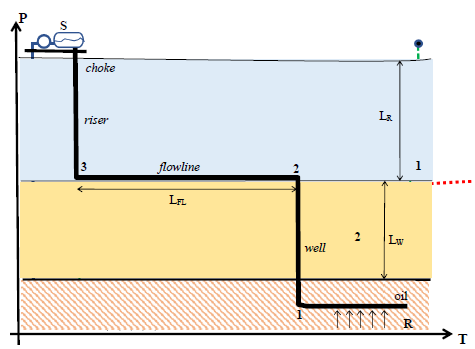
\includegraphics[width=0.9\linewidth]{flow_problem.png}
            \caption{Esquemático das linhas de produção e injeção do problema proposto.}
            \label{fig:desenhoflow}
        \end{figure}

        A bomba de injeção de água tem eficiência de $75\%$. O compressor de exportação de gás tem eficiência politrópica de $76\%$, razão de capacidade térmica do fluido de $1.4$ e pressão de saída de $120\,bar$.

        A perda de gás é de $2\%$ do gás produzido.

        A simulação tem cinco anos de duração. O passo de tempo mínimo é de 0.1 dia e o máximo de 10 dias. O controle de passos de tempo limita a máxima variação da pressão a 5 bar, e de saturação de água a 0.5\%.

    \section{Resultados}

        Algumas conclusões podem ser tiradas dos resultados do modelo integrado proposto:

        \begin{itemize}
            \item As pressões de injeção de água estão muito altas (Figura \ref{fig:pressoespocos}). O modelo integrado precisa de controles adicionais para evitar este tipo de situação. Associado a isto é preciso implementar um modelo de reservatório compressível.
            \item A maior demanda de energia vem da bomba de injeção de água (Figura \ref{fig:demandaenergia}). Um controle na potência da bomba de injeção de água ajudará a reduzir a demanda energética.
            \item A \emph{ESP} tem impacto não desprezível na demanda energética. É preciso otimizar o seu uso e posição de instalação.
            \item A produção de gás é muito baixa, e insuficiente para atender a demanda energética. A exportação de gás é nula e é preciso usar diesel para suprir o excedente da demanda (Figura \ref{fig:emissao}). Para este projeto pode ser importante a busca por fontes alternativas de fornecimento de energia.
            \item A curva de emissão de $CO_2$ por boe produzido (Figura \ref{fig:emissaorel}) mostra primeiro uma redução, associada à entrada de água no reservatório, reduzindo a demanda das bombas de injeção de água. Depois se apresenta um significativo incremento, resultado da chegada de água no produtor. Uma recuperação mais eficiente do óleo se traduz também em menores emissões.
        \end{itemize}

        Gráficos de todos os resultados gerados na solução do problema proposto foram concentrados no \ref{sec:figuras}.

        Em face dos resultados do modelo proposto, foram feitas diferentes sensibilidades com o modelo integrado.

        Foi avaliado o efeito do uso da \emph{ESP}. Observa-se que neste modelo a \emph{ESP} tem efeito negativo na emissão de $CO_2$ (Figura \ref{fig:emissaorelesp}). Na verdade, neste modelo incompressível a \emph{ESP} não tem impacto na produção de óleo. A produção é função unicamente da vazão de injeção de água. Ao usar a \emph{ESP} o efeito é de reduzir a pressão de fundo no produtor, que reduz a pressão de fundo no injetor e que, por último, reduz a demanda de energia na bomba de água (Figura \ref{fig:pwhinjsens}). Como foi assumida uma eficiência menor na \emph{ESP} que na bomba de água, as emissões sobem com o maior uso da \emph{ESP}.

        \begin{figure}[hbt!]
            \begin{tikzpicture}
                \begin{axis}[
                    grid=both,
                    xlabel = {Tempo [$d$]},
                    ylabel = {Emissão [$kgCO_2/boe$]},
                    legend style={at={(0.65,0.82)}, anchor=east, font=\footnotesize},
                    ]
                    \addplot[color=black, solid, thick] table [x=Time_d, y=RelEmission_kgCO2/boe] {results_esp0.0.txt};
                    \addplot[color=red, solid, thick] table [x=Time_d, y=RelEmission_kgCO2/boe] {results_main.txt};
                    \addplot[color=green, solid, thick] table [x=Time_d, y=RelEmission_kgCO2/boe] {results_esp100.0.txt};
                    \legend{$\Delta P = 0\,bar$,$\Delta P = 50\,bar$,$\Delta P = 100\,bar$};
                \end{axis}
            \end{tikzpicture}
            \caption{Emissão de $CO_2$ relativa em função do incremento de pressão da \emph{ESP}.}
            \label{fig:emissaorelesp}
        \end{figure}

        \begin{figure}[hbt!]
            \begin{tikzpicture}
                \begin{axis}[
                    grid=both,
                    xlabel = {Tempo [$d$]},
                    ylabel = {$Pwh_{inj.}\,[bar]$},
                    legend style={font=\footnotesize},
                    ]
                    \addplot[color=black, solid, thick] table [x=Time_d, y=PwhInj_bar] {results_esp0.0.txt};
                    \addplot[color=red, solid, thick] table [x=Time_d, y=PwhInj_bar] {results_main.txt};
                    \addplot[color=green, solid, thick] table [x=Time_d, y=PwhInj_bar] {results_esp100.0.txt};
                    \legend{$\Delta P = 0\,bar$,$\Delta P = 50\,bar$,$\Delta P = 100\,bar$};
                \end{axis}
            \end{tikzpicture}
            \caption{Emissão de $CO_2$ relativa em função do incremento de pressão da \emph{ESP}.}
            \label{fig:pwhinjsens}
        \end{figure}

        Testes com variação no diâmetro dos poços mostrou que o impacto é maior na pressão de fundo do poço produtor (Figuras \ref{fig:pwfprodsensdiametro}) e na de cabeça do injetor (Figura \ref{fig:pwfinjsensdiametro}). O efeito é moderado reflexo nas emissões (Figura \ref{fig:emissaorelsensdiametro}), em função de menor demanda da bomba de injeção de água.

        \begin{figure}[hbt!]
            \begin{tikzpicture}
                \begin{axis}[
                    grid=both,
                    xlabel = {Tempo [$d$]},
                    ylabel = {$Pwf_{prod.}\,[bar]$},
                    legend style={font=\footnotesize},
                    ]
                    \addplot[color=black, solid, thick] table [x=Time_d, y=PwfProd_bar] {results_main.txt};
                    \addplot[color=red, solid, thick] table [x=Time_d, y=PwfProd_bar] {results_d6_prod.txt};
                    \addplot[color=green, solid, thick] table [x=Time_d, y=PwfProd_bar] {results_d6_inj.txt};
                    \legend{Ambos=$4\,pol$, Prod.=$6\,pol$, Inj.=$6\,pol$};
                \end{axis}
            \end{tikzpicture}
            \caption{Efeito dos diâmetros dos poços na pressão de fundo do produtor.}
            \label{fig:pwfprodsensdiametro}
        \end{figure}

        \begin{figure}[hbt!]
            \begin{tikzpicture}
                \begin{axis}[
                    grid=both,
                    xlabel = {Tempo [$d$]},
                    ylabel = {$Pwh_{inj.}\,[bar]$},
                    legend style={font=\footnotesize},
                    ]
                    \addplot[color=black, solid, thick] table [x=Time_d, y=PwhInj_bar] {results_main.txt};
                    \addplot[color=red, solid, thick] table [x=Time_d, y=PwhInj_bar] {results_d6_prod.txt};
                    \addplot[color=green, solid, thick] table [x=Time_d, y=PwhInj_bar] {results_d6_inj.txt};
                    \legend{Ambos=$4\,pol$, Prod.=$6\,pol$, Inj.=$6\,pol$};
                \end{axis}
            \end{tikzpicture}
            \caption{Efeito dos diâmetros dos poços na pressão de cabeça do injetor.}
            \label{fig:pwfinjsensdiametro}
        \end{figure}

        \begin{figure}[hbt!]
            \begin{tikzpicture}
                \begin{axis}[
                    grid=both,
                    xlabel = {Tempo [$d$]},
                    ylabel = {Emissão [$kgCO_2/boe$]},
                    legend style={at={(0.65,0.82)}, anchor=east, font=\footnotesize},
                    ]
                    \addplot[color=black, solid, thick] table [x=Time_d, y=RelEmission_kgCO2/boe] {results_main.txt};
                    \addplot[color=red, solid, thick] table [x=Time_d, y=RelEmission_kgCO2/boe] {results_d6_prod.txt};
                    \addplot[color=green, solid, thick] table [x=Time_d, y=RelEmission_kgCO2/boe] {results_d6_inj.txt};
                    \legend{Ambos=$4\,pol$, Prod.=$6\,pol$, Inj.=$6\,pol$};
                \end{axis}
            \end{tikzpicture}
            \caption{Efeito dos diâmetros dos poços na emissão de $CO_2$.}
            \label{fig:emissaorelsensdiametro}
        \end{figure}

        Em face do impacto do uso de diesel para gerar a energia que o gás disponível não consegue atender, foi avaliado o impacto de usar outras fontes de energia. Uma opção é o uso de diesel verde. Uma página do Departamento de Energia dos Estados Unidos\cite{USDepEnergy} cita dois estudos que apontam para reduções entre 5 e 65\% na quantidade de $CO_2$ emitido pela queima de diesel. Também foi avaliado o impacto do uso de energia de fontes renováveis. Assumiu-se emissões nulas ao usar energia eólica. Observa-se que o impacto nas emissões é significativo (Figura \ref{fig:emissaorelsens}).

        \begin{figure}[hbt!]
            \begin{tikzpicture}
                \begin{axis}[
                    grid=both,
                    xlabel = {Tempo [$d$]},
                    ylabel = {Emissão [$kgCO_2/boe$]},
                    legend style={at={(0.65,0.82)}, anchor=east, font=\footnotesize},
                    ]
                    \addplot[color=black, solid, thick] table [x=Time_d, y=RelEmission_kgCO2/boe] {results_main.txt};
                    \addplot[color=red, solid, thick] table [x=Time_d, y=RelEmission_kgCO2/boe] {results_green_diesel_2.txt};
                    \addplot[color=green, solid, thick] table [x=Time_d, y=RelEmission_kgCO2/boe] {results_green_diesel_1.txt};
                    \addplot[color=blue, solid, thick] table [x=Time_d, y=RelEmission_kgCO2/boe] {results_windfarm.txt};
                    \legend{Diesel, Diesel verde (-5\% $CO_2$), Diesel verde (-65\% $CO_2$), Energia eólica};
                \end{axis}
            \end{tikzpicture}
            \caption{Emissão de $CO_2$ relativa em função da fonte de energia utilizada.}
            \label{fig:emissaorelsens}
        \end{figure}

        O código foi implementado em Python e pode ser encontrado em \href{https://github.com/TiagoCAAmorim/IntegratedModel/}{https://github.com/TiagoCAAmorim/Integra tedModel/}.

    \section{Conclusão}
        Foi implementado um conjunto de classes que representam diferentes sistemas de um modelo integrado. O acoplamento realizado se mostrou suficiente para as análises pretendidas.
        Os resultados mostraram que é preciso avaliar as decisões de projeto com vista não somente na recuperação de óleo, mas também em termos de emissões de $CO_2$.

    % \label{}

%% The Appendices part is started with the command \appendix;
%% appendix sections are then done as normal sections

\appendix

    \section{Lista de Variáveis}

        \begin{description}
            \item[$^oAPI$:]Grau API do óleo.
            \item[$\beta$:]Constante de ajuste da eficiência energética.
            \item[$Bp$:]Fator volume de formação da fase $p$ no reservatório ($m^3/m^3$).
            \item[$c_o$:]Compressibilidade do óleo ($1/bar$).
            \item[$D$:]Profundidade.
            \item[$d$:]Diâmetro da tubulação ($m$).
            \item[$dp$:]Densidade relativa da fase $p$.
            \item[$\Delta x$:]Discretização espacial na direção $i$.
            \item[$\Delta y$:]Discretização espacial na direção $j$.
            \item[$\Delta z$:]Discretização espacial na direção $k$.
            \item[$\Delta t$:]Discretização temporal.
            \item[$\eta$:]Eficiência energética.
            \item[$\gamma_p$:]Peso específico da fase $p$ ($\gamma_p = \rho_p g$).
            \item[$\dot{\gamma}$:]Taxa de cisalhamento ($1/s$).
            \item[$k$:]Permeabilidade absoluta do meio poroso.
            \item[$k_{rp}$:]Permeabilidade relativa da fase $p$.
            \item[$\mu_p$:]Viscosidade da fase $p$.
            \item[$p_p$:]Pressão da fase $p$.
            \item[$Pwf$:]Pressão de fluxo no fundo do poço (\emph{Bottom-hole pressure}).
            \item[$Pwh$:]Pressão de cabeça do poço (\emph{Wellhead pressure}).
            \item[$\phi$:]Porosidade da rocha.
            \item[$q_p$:]Vazão volumétrica da fase $p$.
            \item[$q^w_{cp}$:]Vazão mássica do componente $c$ na fase $p$.
            \item[$q^{std}_{cp}$:]Vazão volumétrica da fase $p$ medida em condições padrão (\emph{standard}).
            \item[$RGO$]Razão gás-óleo em condições de superfície ($m^3/m^3$).
            \item[$\rho_p$:]Densidade da fase $p$.
            \item[$S_p$:]Saturação da fase $p$ no meio poroso.
            \item[$V$:]Volume total do volume de controle (célula).
            \item[$wcut$:]Corte de água ($Qw/(Qw+Qo)$).
            \item[$v_p$:]Velocidade da fase $p$.
            \item[$y_{cp}$:]Concentração do componente $c$ na fase $p$.
        \end{description}

    \section{Resultados do Modelo Proposto} \label{sec:figuras}

        \begin{figure}[H]
            \begin{tikzpicture}
                \begin{axis}[
                    grid=both,
                    xlabel = {Tempo [$d$]},
                    ylabel = {Passo de Tempo [$d$]},
                    ]
                    \addplot[color=blue, solid, thick] table [x=Time_d, y=TimeStep_d] {results_main.txt};
                \end{axis}
            \end{tikzpicture}
            \caption{Passos de tempo.}
            \label{fig:deltat}
        \end{figure}

        \begin{figure}[H]
            \begin{tikzpicture}
                \begin{axis}[
                    grid=both,
                    xlabel = {Tempo [$d$]},
                    ylabel = {Vazão [$m^3/d$]},
                    legend style={at={(0.90,0.50)}, anchor=east, font=\footnotesize},
                    ]
                    \addplot[color=green, solid, thick] table [x=Time_d, y=Qo_m3/d] {results_main.txt};
                    \addplot[color=blue, solid, thick] table [x=Time_d, y=Qw_m3/d] {results_main.txt};
                    \addplot[color=black, solid, thick] table [x=Time_d, y=Qwi_m3/d] {results_main.txt};
                    \legend{Qo, Qw, Qwi};
                \end{axis}
            \end{tikzpicture}
            \caption{Vazão de óleo e água.}
            \label{fig:vazao}
        \end{figure}

        \begin{figure}[H]
            \begin{tikzpicture}
                \begin{axis}[
                    grid=both,
                    xlabel = {Tempo [$d$]},
                    ylabel = {Vazão [$m^3/d$]},
                    legend style={font=\footnotesize},
                    ]
                    \addplot[color=red, solid, thick] table [x=Time_d, y=Qg_m3/d] {results_main.txt};
                    \addplot[color=black, solid, thick] table [x=Time_d, y=QgFlare_m3/d] {results_main.txt};
                    \addplot[color=green, solid, thick] table [x=Time_d, y=QgFuel_m3/d] {results_main.txt};
                    \addplot[color=blue, solid, thick] table [x=Time_d, y=QgExp_m3/d] {results_main.txt};
                    \legend{Produção, \emph{Flare}, Combustível, Exportação};
                \end{axis}
            \end{tikzpicture}
            \caption{Gerenciamento do gás.}
            \label{fig:gerenciamentogas}
        \end{figure}

        \begin{figure}[H]
            \begin{tikzpicture}
                \begin{axis}[
                    grid=both,
                    xlabel = {Tempo [$d$]},
                    ylabel = {Pressão [$bar$]},
                    legend style={font=\footnotesize},
                    ]
                    \addplot[color=green, solid, thick] table [x=Time_d, y=PwfProd_bar] {results_main.txt};
                    \addplot[color=blue, solid, thick] table [x=Time_d, y=PwfInj_bar] {results_main.txt};
                    \addplot[color=green, dashed, thick] table [x=Time_d, y=PwhProd_bar] {results_main.txt};
                    \addplot[color=blue, dashed, thick] table [x=Time_d, y=PwhInj_bar] {results_main.txt};
                    \legend{$Pwf_{prod.}$, $Pwf_{inj.}$, $Pwh_{prod.}$, $Pwh_{inj.}$};
                \end{axis}
            \end{tikzpicture}
            \caption{Pressões de fundo e de cabeça dos poços.}
            \label{fig:pressoespocos}
        \end{figure}

        \begin{figure}[H]
            \begin{tikzpicture}
                \begin{axis}[
                    grid=both,
                    xlabel = {Tempo [$d$]},
                    ylabel = {Energia [$MW$]},
                    legend style={font=\footnotesize},
                    ]
                    \addplot[color=red, solid, thick] table [x=Time_d, y=Pump_MW] {results_main.txt};
                    \addplot[color=black, solid, thick] table [x=Time_d, y=ESP_MW] {results_main.txt};
                    \addplot[color=green, solid, thick] table [x=Time_d, y=ExpCompr_MW] {results_main.txt};
                    \addplot[color=blue, solid, thick] table [x=Time_d, y=TotalPower_MW] {results_main.txt};
                    \legend{Bomba de água, \emph{ESP}, Exportação, Total};
                \end{axis}
            \end{tikzpicture}
            \caption{Demanda energética.}
            \label{fig:demandaenergia}
        \end{figure}

        \begin{figure}[H]
            \begin{tikzpicture}
                \begin{axis}[
                    grid=both,
                    xlabel = {Tempo [$d$]},
                    ylabel = {Emissão [$tonCO_2/d$]},
                    legend style={font=\footnotesize},
                    ]
                    \addplot[color=red, solid, thick] table [x=Time_d, y=GasEmission_tonCO2/d] {results_main.txt};
                    \addplot[color=blue, solid, thick] table [x=Time_d, y=DieselEmission_tonCO2/d] {results_main.txt};
                    \addplot[color=black, solid, thick] table [x=Time_d, y=TotalEmission_tonCO2/d] {results_main.txt};
                    \legend{Gás Combustível, Diesel, Total};
                \end{axis}
            \end{tikzpicture}
            \caption{Emissão de $CO_2$.}
            \label{fig:emissao}
        \end{figure}

        \begin{figure}[H]
            \begin{tikzpicture}
                \begin{axis}[
                    grid=both,
                    xlabel = {Tempo [$d$]},
                    ylabel = {Emissão [$tonCO_2$]},
                    ]
                    \addplot[color=black, solid, thick] table [x=Time_d, y=CumEmission_tonCO2] {results_main.txt};
                \end{axis}
            \end{tikzpicture}
            \caption{Emissão de $CO_2$ acumulada.}
            \label{fig:emissaocum}
        \end{figure}

        \begin{figure}[H]
            \begin{tikzpicture}
                \begin{axis}[
                    grid=both,
                    xlabel = {Tempo [$d$]},
                    ylabel = {Emissão [$kgCO_2/boe$]},
                    ]
                    \addplot[color=black, solid, thick] table [x=Time_d, y=RelEmission_kgCO2/boe] {results_main.txt};
                \end{axis}
            \end{tikzpicture}
            \caption{Emissão de $CO_2$ relativa.}
            \label{fig:emissaorel}
        \end{figure}
%
%  	   RelEmission_kgCO2/boe

%% \section{}
%% \label{}

%% If you have bibdatabase file and want bibtex to generate the
%% bibitems, please use
%%

\bibliographystyle{elsarticle-num}
\bibliography{refs}

%% else use the following coding to input the bibitems directly in the
%% TeX file.

% \begin{thebibliography}{00}

%% \bibitem{label}
%% Text of bibliographic item

% \bibitem{}

% \end{thebibliography}

% \newpage
% \FloatBarrier
% \section{Código em C}

% O código de ambos métodos foi implementado em um único arquivo. O código é apresentado em duas partes neste documento para facilitar a leitura. O código pode ser encontrado em \href{https://github.com/TiagoCAAmorim/numerical-methods}{https://github.com/TiagoCAAmorim/numerical-methods}.

% \subsection{Método da Bissecção}
% \lstinputlisting[language=C, linerange={1-229}]{./02_newton_raphson.c}

% \subsection{Método de Newton-Raphson}
% \lstinputlisting[language=C, linerange={231-445}]{./02_newton_raphson.c}

% \subsection{Método da Mínima Curvatura}
% \lstinputlisting[language=C, linerange={448-958}]{./02_newton_raphson.c}

\end{document}
\endinput